% !TEX root =  main.tex

\section{The DARC Toolbox}
\label{sec:design:darc}

We now demonstrate the utility of our approach by considering its application 
to automating the adaptive design psychology experiments via the DARC (Delay
And Risky Choice) toolbox introduced in~\cite{vincent2017darc}.\footnote{Code available at~ \url{http://github.com/drbenvincent/darc-experiments-matlab}.}  We will only provide
a short introduction here and refer the reader to~\cite{vincent2017darc} for further details.

The DARC toolbox allows users 
to encode their own (or use one of the provided) models for human \emph{discounting} behavior,
whereby psychologists want to learn how delays and uncertainties affect the subjective value people place
on (typically monetary) rewards or costs. Given a model, the toolbox uses the framework from the
previous section to automate in an online fashion 
both the inference of the model parameters and the sequential adaptation of the experiment itself through
choosing the questions the participant is asked.  It, therefore, automates the full run-time experimental 
pipeline  by using the responses from previous questions to perform inference 
and update the internal representation
of the participant and then using this information to ask the most informative questions for a particular
participant as per the BED equations.  The technical innovations introduced earlier in this chapter
are essential in allowing this to be done sufficiently efficiently to permit
real-time usage required for deployment with real participants.

\begin{figure}[t]
	\centering
	\begin{subfigure}[b]{0.49\textwidth}
		\centering
		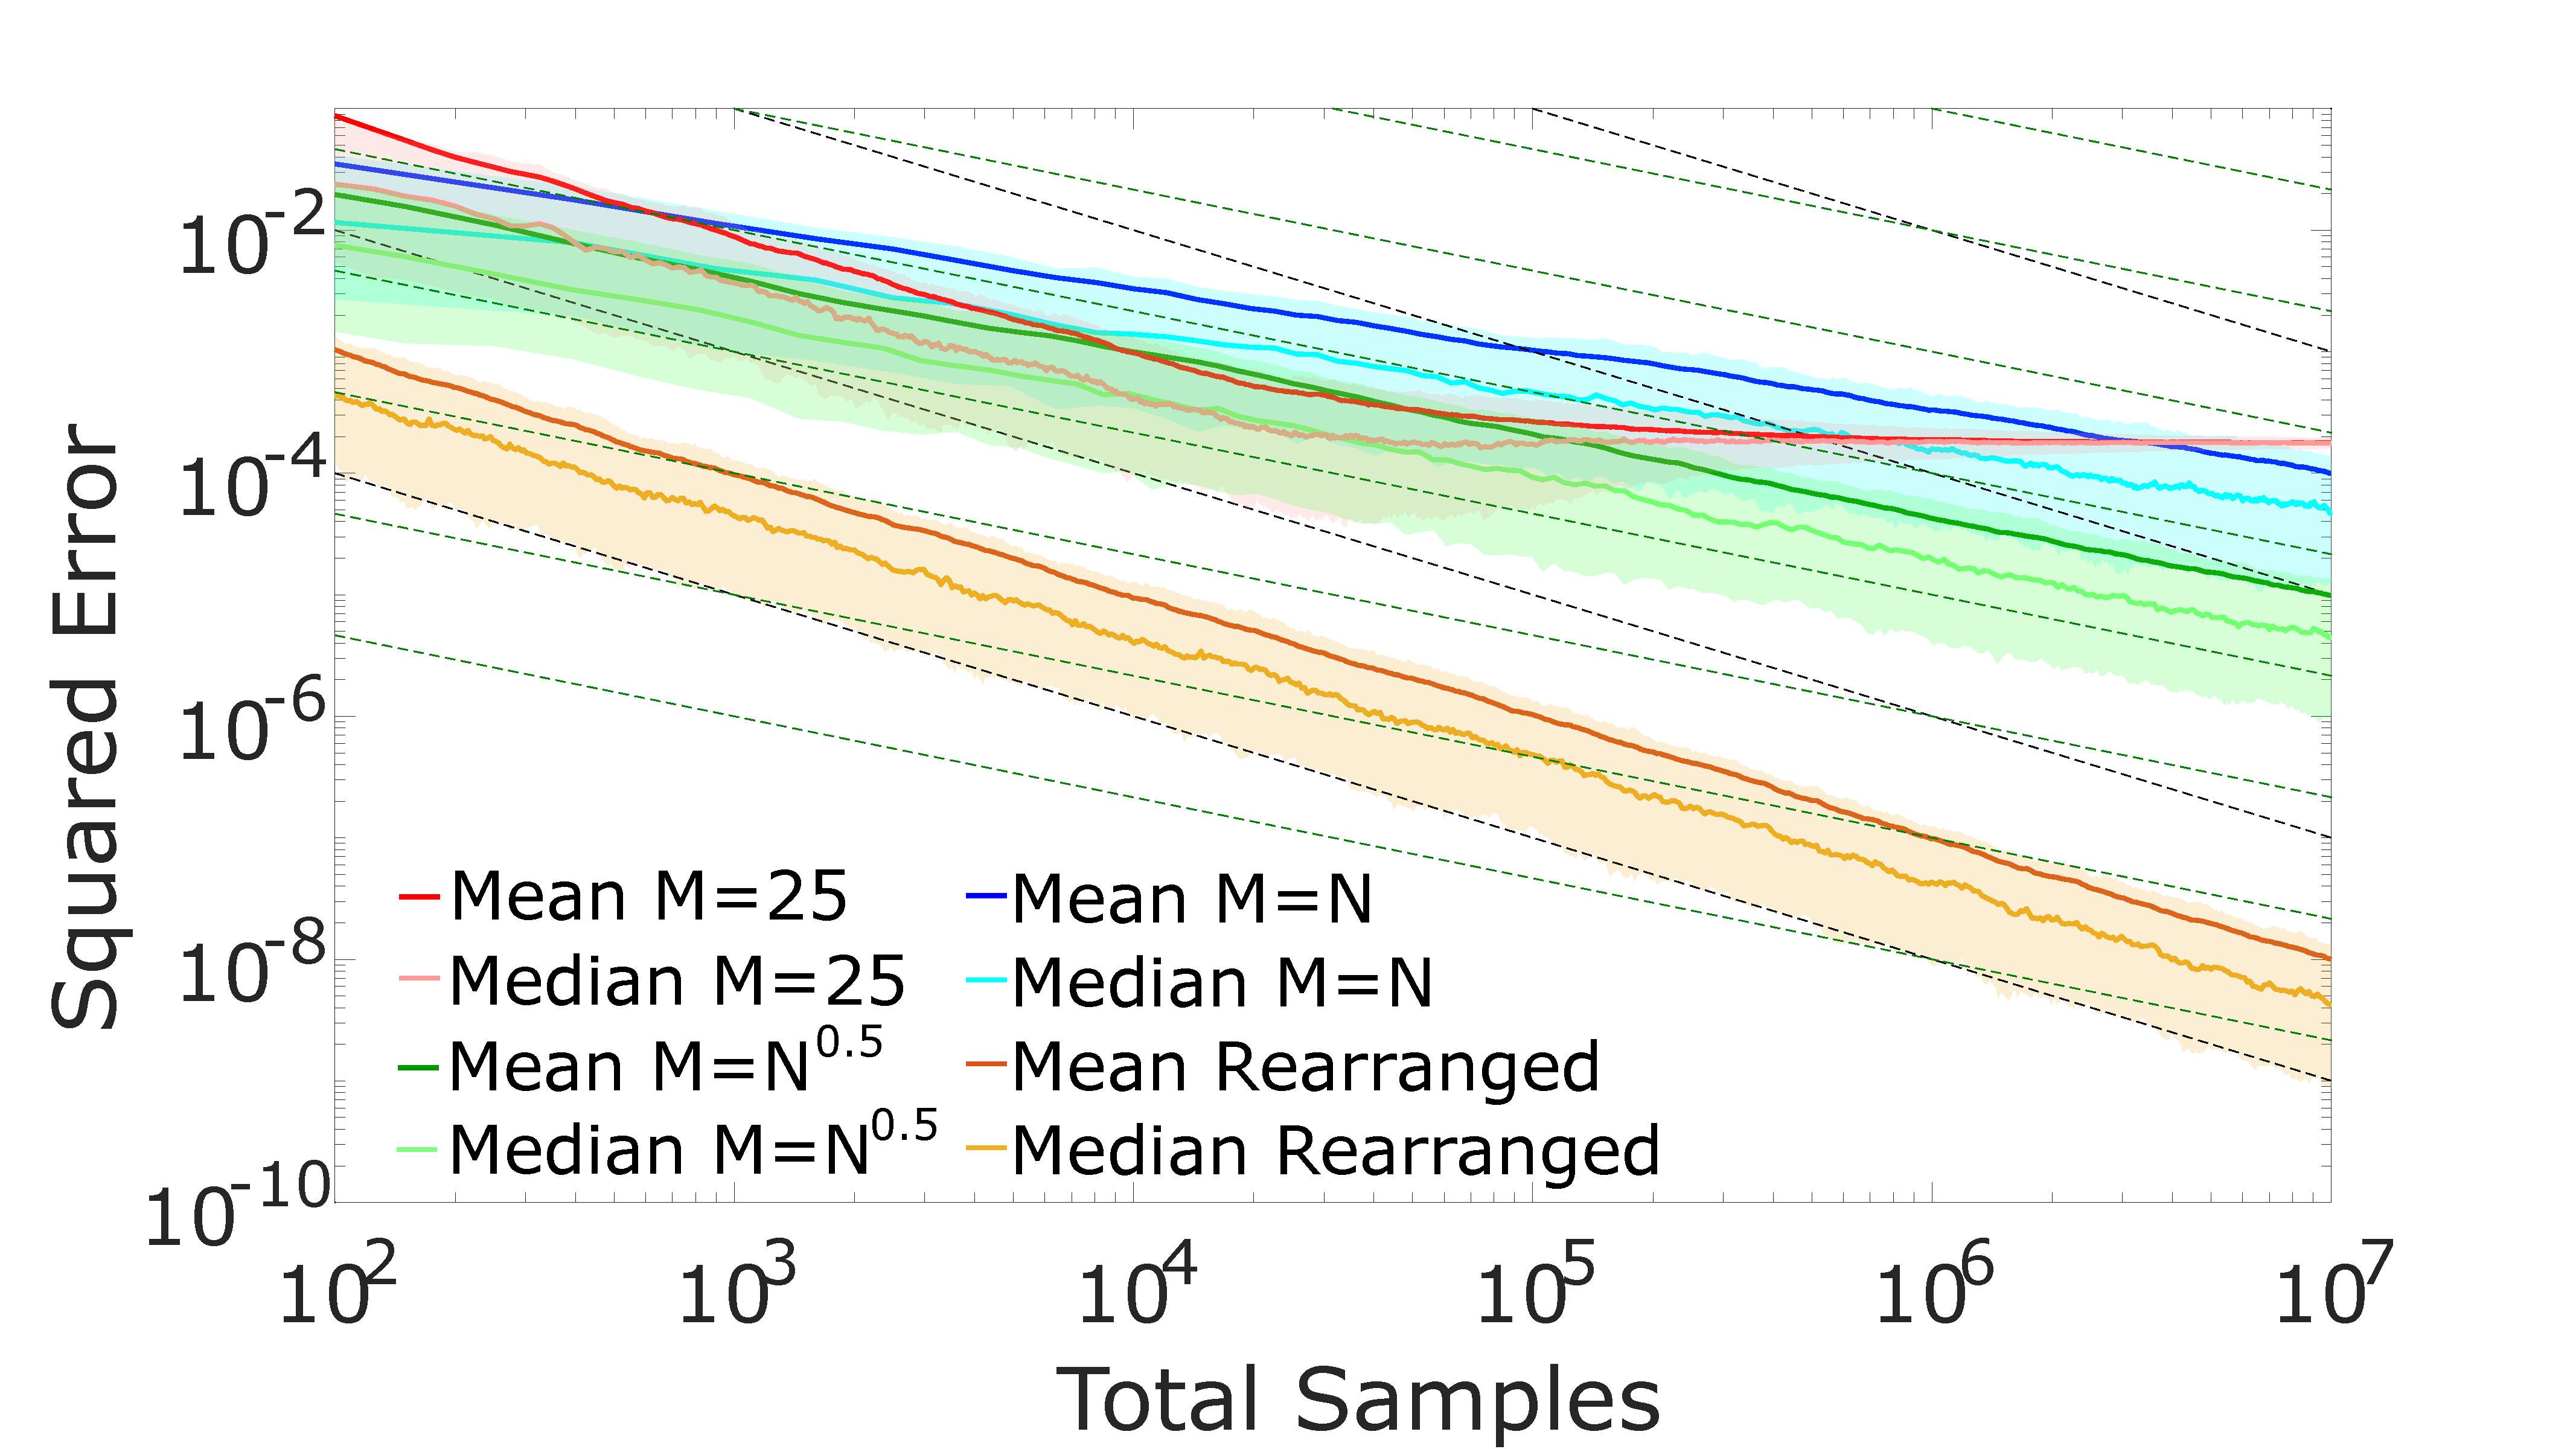
\includegraphics[width=0.99\textwidth,trim={1.5cm 0 3.5cm 0},clip]{exp_conv2}
		\caption{Convergence of BED\label{fig:exp-conv}}
	\end{subfigure}
		\begin{subfigure}[b]{0.49\textwidth}
			\centering
			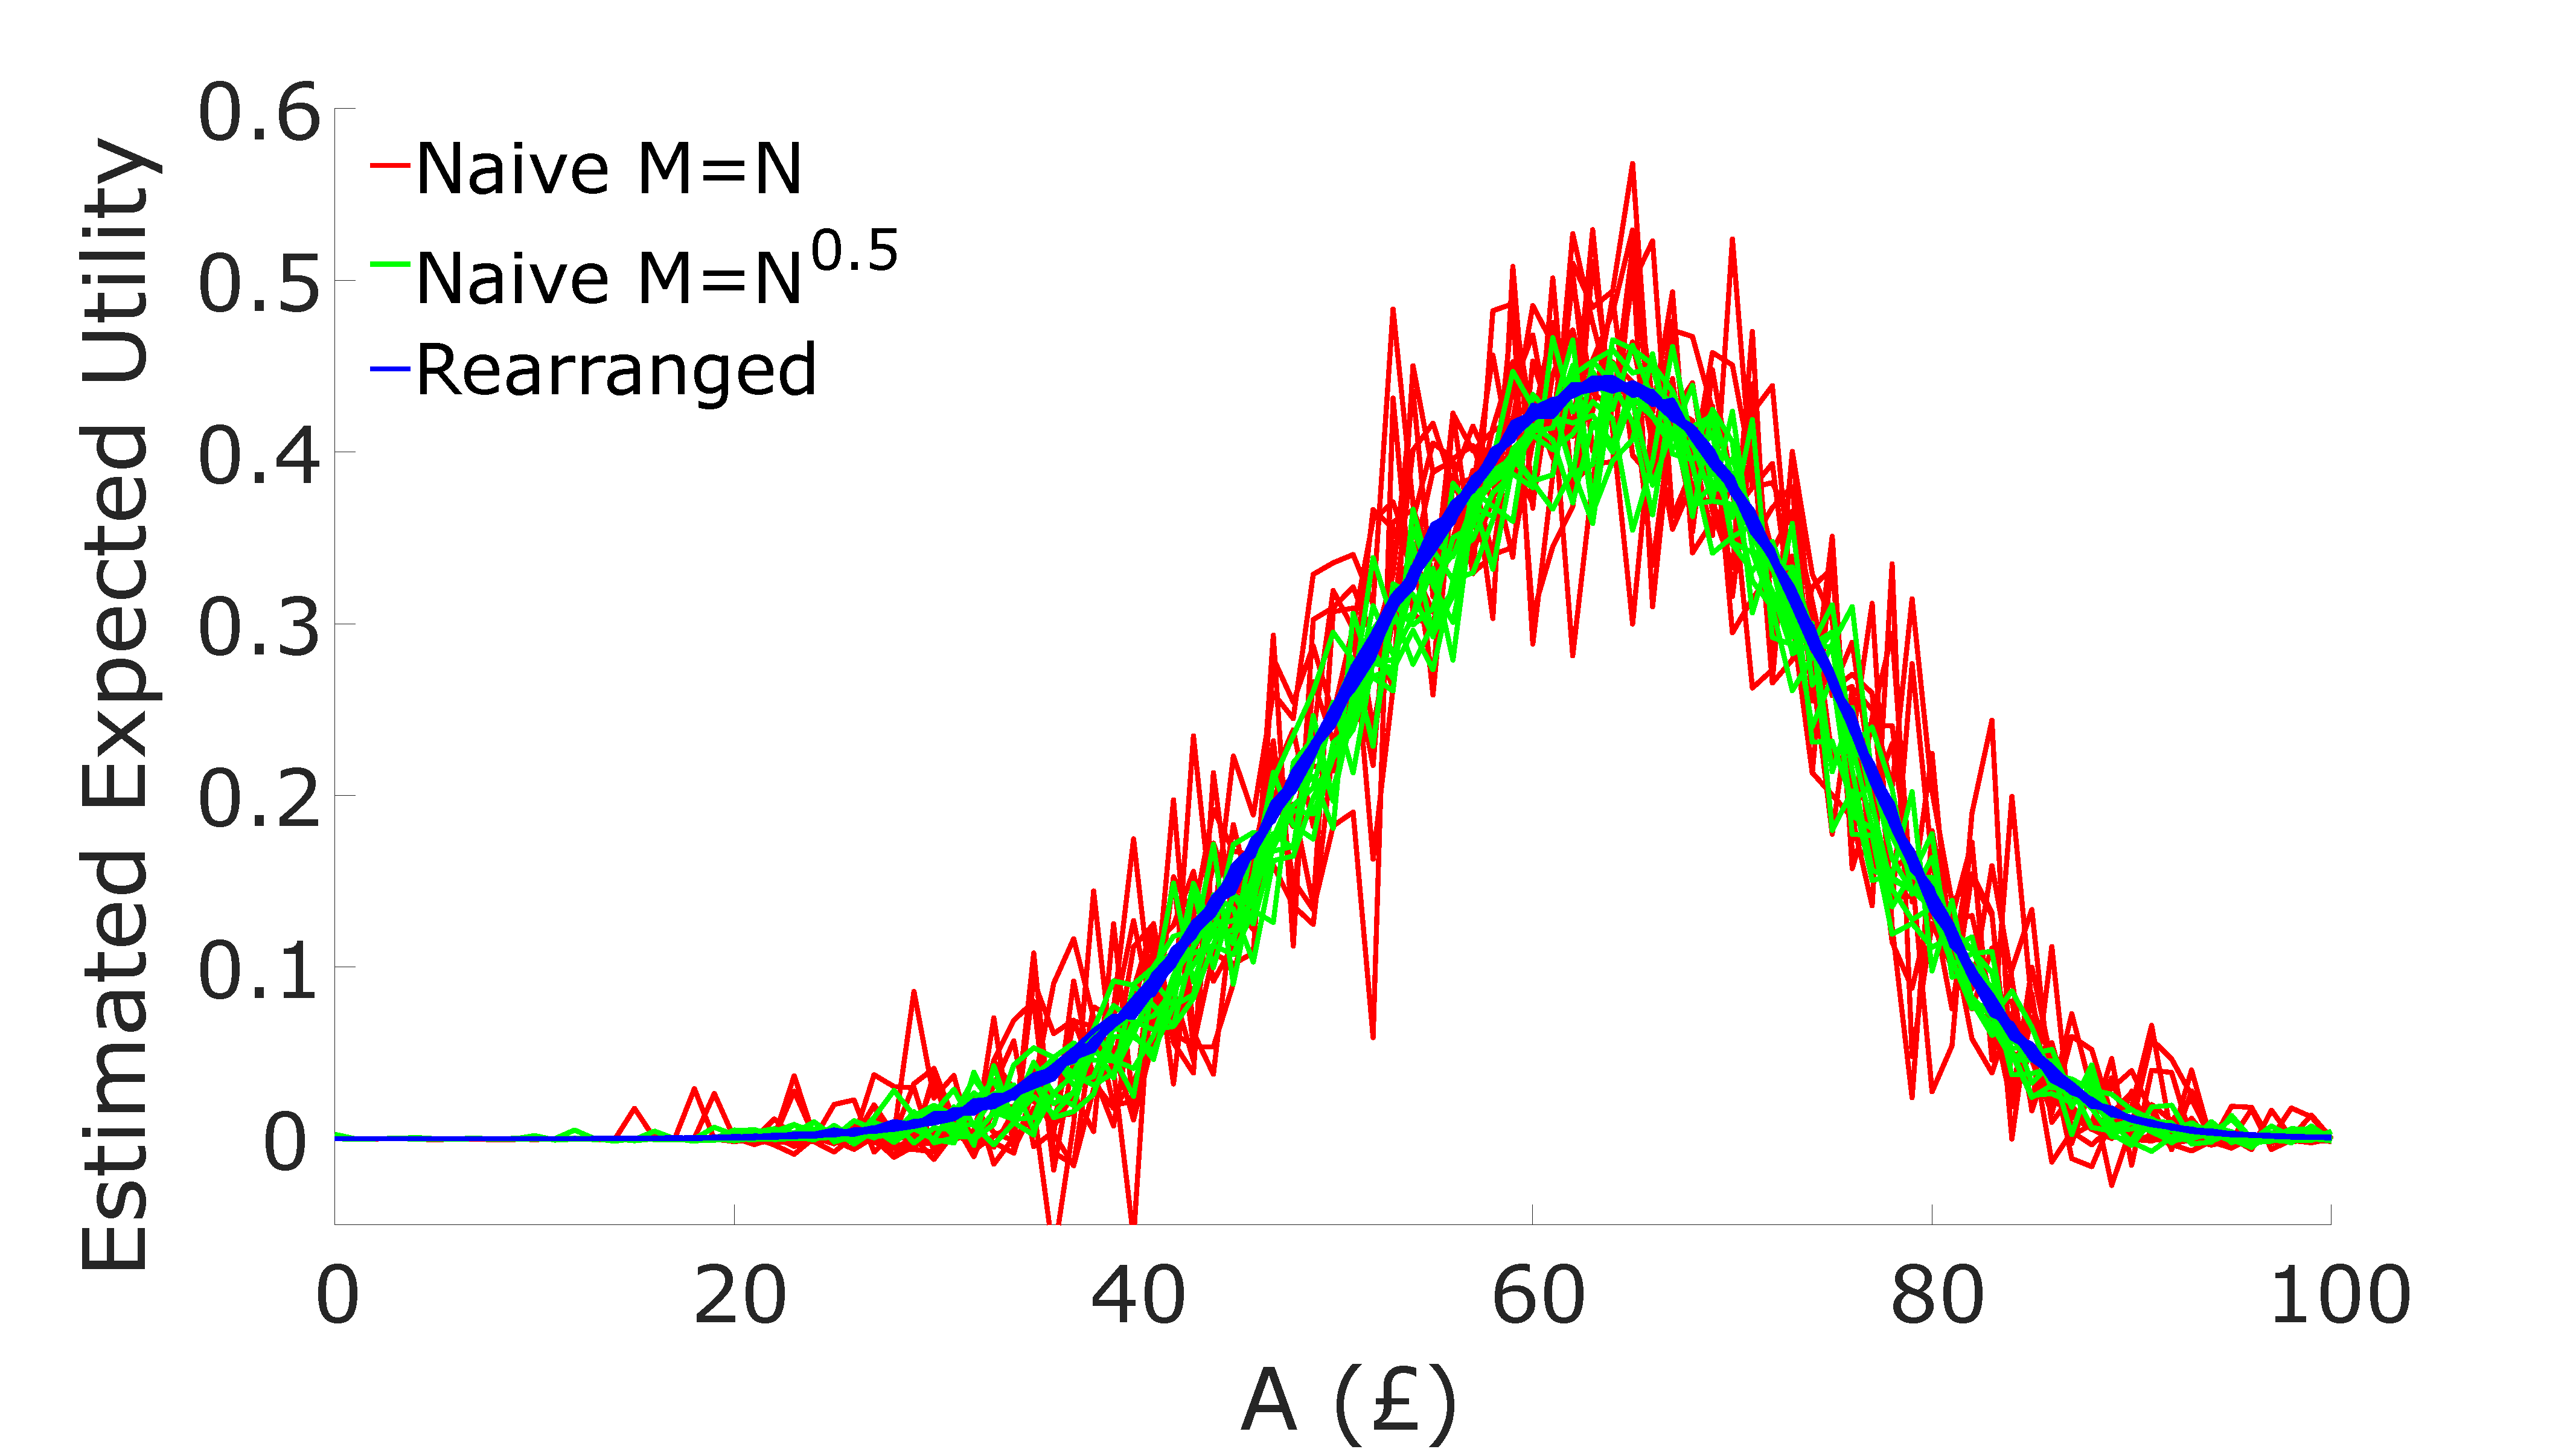
\includegraphics[width=0.99\textwidth,trim={1.5cm 0 3.5cm 0},clip]{dscan_2}
			\caption{Estimated expected utilities \label{fig:exp-d-scan}}
		\end{subfigure}
		\vspace{5pt}
	\caption{(Left) convergence of both NMC and our reformulated
		estimator~\eqref{eq:u_bar_MC} for the BED problem.
		A ground truth estimate was calculated using a single run of the reformulated
		estimator with $10^{10}$ samples.
		Results are averaged over 1000 independent runs, while shaded regions give the 25\%-75\% quantiles. We
		see that the theoretical convergence rates (shown by the dashed lines) are observed in all cases,
		with the advantages of the reformulated estimator particularly pronounced.
		(Right) estimated expected utilities $\bar{U}(d)$for 
		different values of one of the design parameters $A \in \{1,2,\dots,100\}$ given a fixed total
		sample budget of $T=10^4$.  Here the lines correspond to 10 independent runs, showing
		that the variance of \eqref{eq:exp-des-nmc} is far higher than \eqref{eq:u_bar_MC}.
		}
\end{figure}

A common style of experiment for the toolbox comprises of asking questions of the form 
\emph{``Would you prefer $\pounds A$ now, or $\pounds B$ in $D^b$ days?''}, where we desire
to choose the question  variables $d = \{A,B,D^b\}$ in the manner that will give the most 
incisive questions.  One possible participant model, given in ~\citep{vincent2016hierarchical},
presumes that participants have parameters $\theta=\{\log k,\alpha\}$, where $\log k \sim \mathcal{N}(-4.5,0.5^2)$ 
represents a $\log$ discount rate and $\alpha\sim \textsc{Gamma}(2,0.5)$ (using the shape-rate parameterization) a variability, and the following response model
\begin{equation}
\label{eq:design:darc}
y \sim \mathrm{Bernoulli} \left(0.01 + 0.98 \; \Phi\left(\frac{1}{\alpha} \left(\frac{B}{1+k D^b}-A\right)\right)\right)
\end{equation}
where $y=1$ indicates choosing the delayed response and $\Phi$ represents the 
cumulative normal distribution. As more questions are asked, the distribution 
over the parameters $\theta$ is updated in the standard Bayesian fashion, such
that the most optimal question to ask at a particular time depends on the previous questions
and responses.  

Before considering the full BED pipeline, we will first examine the convergence and empirical
performance of our
reformulated estimator~\eqref{eq:u_bar_MC}  compared to the na\"{i}ve alternative~\eqref{eq:exp-des-nmc}.
For simplicity, we will consider the case 
where $B=100$ and $D^b = 50$ are fixed and we are only choosing the delayed value $A$.
We first examine the convergence in the estimate of $\bar{U}(d)$ for the case $A=70$,
for which Figure~\ref{fig:exp-conv} demonstrates similar behavior for the na\"{i}ve NMC estimator
as seen in the experiments of Chapter~\ref{chp:nest} and, as expected, substantial improvements
for the reformulated estimator in the form of a $O(1/N)$ convergence rate.

We next consider setting a total sample budget $T=10^4$ and look at the variation in the 
estimated values of $\bar{U}(d)$ for different values of $A$ for the two methods as 
shown in Figure~\ref{fig:exp-d-scan}. This shows that the improvement in MSE leads 
to clearly visible improvements in the characterization of $\bar{U}(d)$ that
will translate to improvements in seeking the optimum.

\begin{figure}[t]
	\centering
		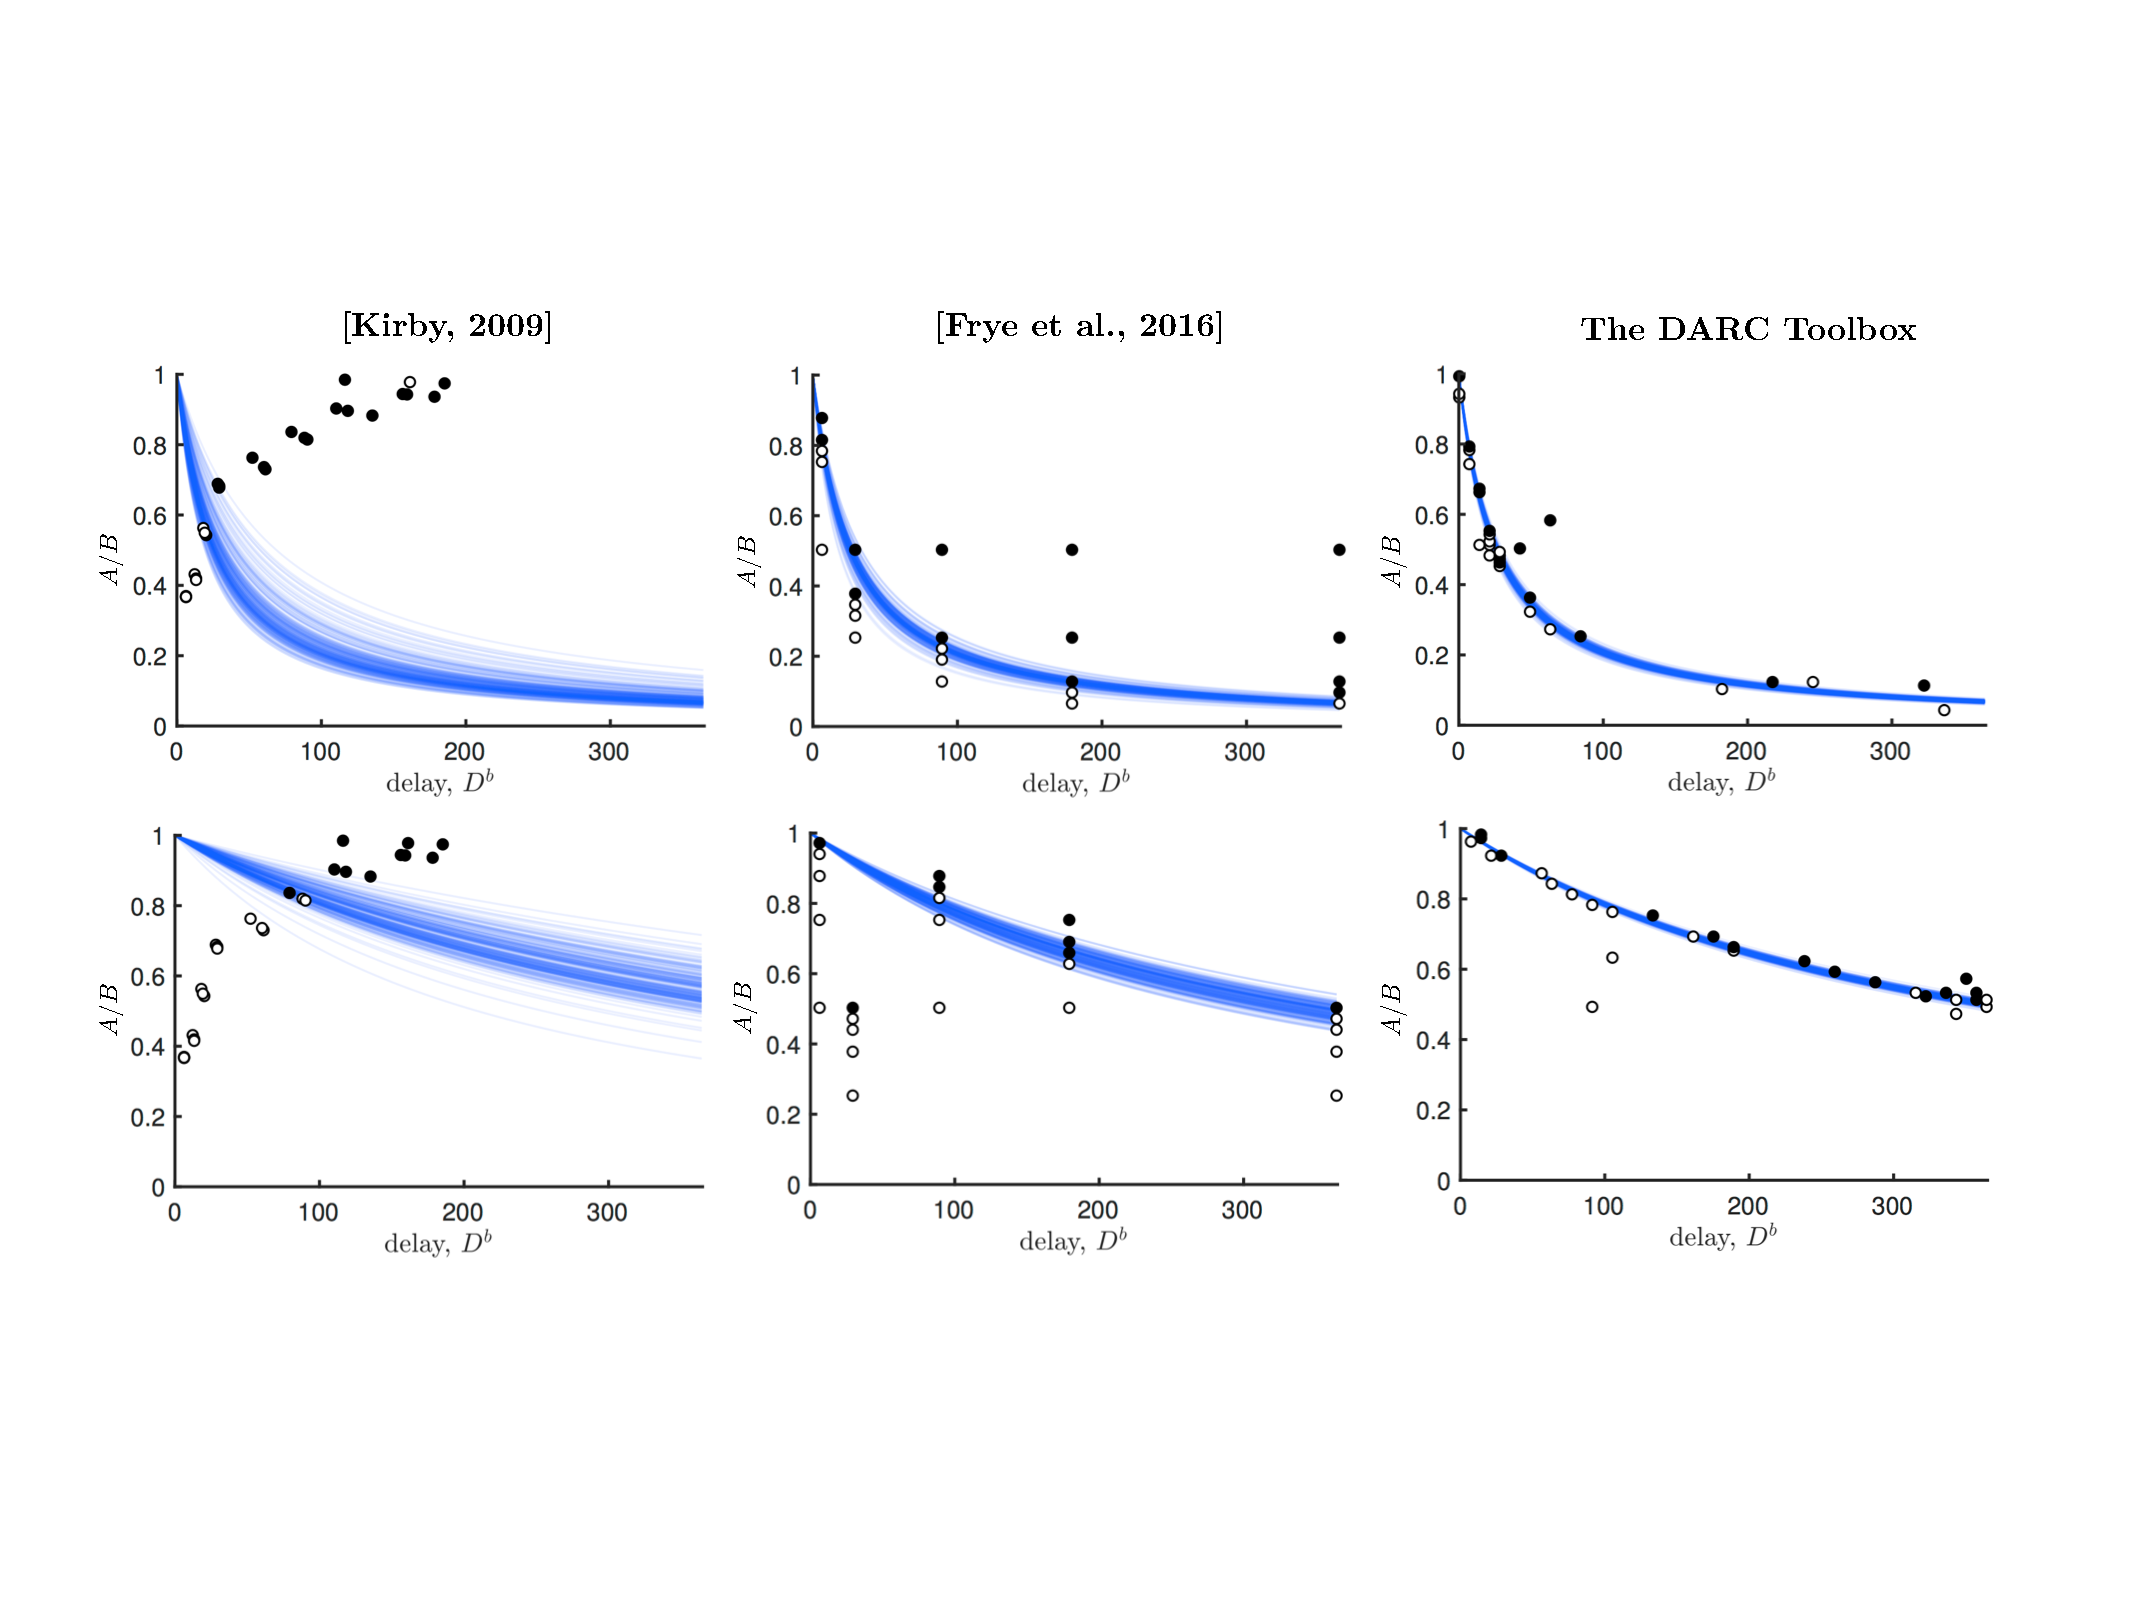
\includegraphics[width=\textwidth]{darc_results}
	\caption{Comparison of the DARC toolbox to alternative methods for two behavior styles: major
		depressive disorder (top) which indicates a relatively strong desire for immediate rewards ($k=0.04$)
		and anorexia nervosa (bottom) which indicates relatively low discounting rate ($k=0.0028$).  Lines show
		posterior samples from the final learned predictive distribution for the indifference curve (i.e. the curve
		along which the participant is equally likely to choose the immediate or delayed reward), circles represent
		questions where the delayed reward was preferred, and the filled dots correspond to the questions were
		the immediate reward was preferred.  The columns left to right corresponding to using the approaches
		of~\cite{Kirby:2009eu} which uses pre-fixed questions rather than using online adaptation,~\cite{Frye:2016eu}
		which uses a heuristic approach for choosing the best questions adaptively, and using our DARC toolbox
		which chooses questions using our sequential BED approach.  See~\cite{vincent2017darc} for further details.
		\label{fig:design:darc}
	}
\end{figure}

Finally, we examine the performance of the DARC toolbox compared to alternatives in the
psychology literature~\citep{Kirby:2009eu,Frye:2016eu} as shown in Figure~\ref{fig:design:darc}.  Using the
same likelihood model as~\eqref{eq:design:darc},
we fix $\alpha=2$ and set the prior on $k$ as $\log k \sim \mathcal{N}(-4.5,0.5^2)$.  We fixed $B=100$ and
then use three different methods for sequentially selecting designs $d_t = \{A_t,D^b_t\}$, for
two different hypothetical participants with respective ground truth parameters of $k=0.04$ and $k=0.0028$.
Responses are generated presuming the likelihood model is correct and sampling directly from
\eqref{eq:design:darc} using the ground truth parameters.  We then plot a characterization of the posterior
predictive after $27$ questions have been asked.  All methods are capable of working in real time, taking
about a second or less to choose the design at each iteration when run on a mid-range laptop.  Though 
hardly a rigorous performance assessment, these results are still demonstrative of the potential utility of our
method.  The non-adaptive scheme of~\cite{Kirby:2009eu} always asks the same questions regardless of
the participant's responses.  The heuristic method of~\cite{Frye:2016eu} does better, but is still somewhat
wasteful.  The DARC toolbox, on the other hand, takes only a couple of questions before achieving a
reasonable representation of the response surface, such that almost all of the questions asked are clearly
pertinent and the final posterior predictive distribution has far lower entropy than the other approaches.